\documentclass[onecolumn, compsoc,11pt]{IEEEtran}
\usepackage{enumitem}
\usepackage{etex}
\usepackage{amssymb,amsfonts,amsmath,amsthm}
\usepackage{graphicx}
%\usepackage[usenames,x11names, dvipsnames, svgnames]{xcolor}
\usepackage{amsmath,amssymb}
\usepackage{dsfont}
\usepackage{amsfonts}
\usepackage{mathrsfs}
\usepackage{array}
\usepackage{xr}
\usepackage{multirow}
%\usepackage{multirow}    
%\usepackage[T1,euler-digits]{eulervm}
%\usepackage{times}
%\usepackage{pxfonts}
\usepackage{tikz}
\usepackage{pgfplots}
\usetikzlibrary{shapes,calc,shadows,fadings,arrows,decorations.pathreplacing,automata,positioning}
\usetikzlibrary{external}
\usetikzlibrary{decorations.text}
\usepgfplotslibrary{colorbrewer} 

\tikzexternalize[prefix=./Figures/External/]% activate externalization!
\tikzexternaldisable
%\addtolength{\voffset}{.1in}  
 \definecolor{nodecol}{RGB}{240,240,220}
 \definecolor{nodeedge}{RGB}{240,240,225}
  \definecolor{edgecol}{RGB}{130,130,130}
    \tikzset{%
fshadow/.style={      preaction={
         fill=black,opacity=.3,
         path fading=circle with fuzzy edge 20 percent,
         transform canvas={xshift=1mm,yshift=-1mm}
       }} 
}
\usetikzlibrary{pgfplots.dateplot}
 \usetikzlibrary{patterns}
\usetikzlibrary{decorations.markings}
\usepackage{mathtools}
\usepackage{datetime}
%% ## Equation Space Control---------------------------
\def\EQSP{5pt}
\newcommand{\mltlne}[2][\EQSP]{\begingroup\setlength\abovedisplayskip{#1}\setlength\belowdisplayskip{#1}\begin{equation}\begin{multlined} #2 \end{multlined}\end{equation}\endgroup\noindent}
\newcommand{\cgather}[2][\EQSP]{\begingroup\setlength\abovedisplayskip{#1}\setlength\belowdisplayskip{#1}\begin{gather} #2 \end{gather}\endgroup\noindent}
\newcommand{\cgathers}[2][\EQSP]{\begingroup\setlength\abovedisplayskip{#1}\setlength\belowdisplayskip{#1}\begin{gather*} #2 \end{gather*}\endgroup\noindent}
\newcommand{\calign}[2][\EQSP]{\begingroup\setlength\abovedisplayskip{#1}\setlength\belowdisplayskip{#1}\begin{align} #2 \end{align}\endgroup\noindent}
\newcommand{\caligns}[2][\EQSP]{\begingroup\setlength\abovedisplayskip{#1}\setlength\belowdisplayskip{#1}\begin{align*} #2 \end{align*}\endgroup\noindent}
\newcommand{\mnp}[2]{\begin{minipage}{#1}#2\end{minipage}} 
%% COLOR DEFS------------------------------------------
\newtheorem{thm}{Theorem}
\newtheorem{cor}{Corollary}
\newtheorem{lem}{Lemma}
\newtheorem{prop}{Proposition}
\newtheorem{defn}{Definition}
\newtheorem{exmpl}{Example}
\newtheorem{rem}{Remark}
\newtheorem{notn}{Notation}
%%------------PROOF INCLUSION -----------------
\def\NOPROOF{Proof omitted.}
\newif\ifproof
\prooffalse % or \draftfalse
\newcommand{\Proof}[1]{
\ifproof
\begin{IEEEproof}
#1\end{IEEEproof}
\else
\NOPROOF
\fi
 }
%%------------ -----------------
\newcommand{\DETAILS}[1]{#1}
%%------------ -----------------
% color commands------------------------
%\newcommand{\etal}{\textit{et} \mspace{3mu} \textit{al.}}
% \renewcommand{\algorithmiccomment}[1]{$/** $ #1 $ **/$}
\newcommand{\vect}[1]{\textbf{\textit{#1}}}
\newcommand{\figfont}{\fontsize{8}{8}\selectfont\strut}
\newcommand{\hlt}{ \bf \sffamily \itshape\color[rgb]{.1,.2,.45}}
\newcommand{\pitilde}{\widetilde{\pi}}
\newcommand{\Pitilde}{\widetilde{\Pi}}
\newcommand{\bvec}{\vartheta}
\newcommand{\algo}{\textrm{\bf\texttt{GenESeSS}}\xspace}
\newcommand{\xalgo}{\textrm{\bf\texttt{xGenESeSS}}\xspace}
\newcommand{\FNTST}{\bf }
\newcommand{\FNTED}{\color{darkgray} \scriptsize $\phantom{.}$}
\renewcommand{\baselinestretch}{.95}
\newcommand{\sync}{\otimes}
\newcommand{\psync}{\hspace{3pt}\overrightarrow{\hspace{-3pt}\sync}}
%\newcommand{\psync}{\raisebox{-4pt}{\begin{tikzpicture}\node[anchor=south] (A) {$\sync$};
%\draw [->,>=stealth] ([yshift=-2pt, xshift=2pt]A.north west) -- ([yshift=-2pt]A.north east); %\end{tikzpicture}}}
\newcommand{\base}[1]{\llbracket #1 \rrbracket}
\newcommand{\nst}{\textrm{\sffamily\textsc{Numstates}}}
\newcommand{\HA}{\boldsymbol{\mathds{H}}}
\newcommand{\eqp}{ \vartheta }
\newcommand{\entropy}[1]{\boldsymbol{h}\left ( #1 \right )}
\newcommand{\norm}[1]{\left\lVert #1 \right\rVert}%
\newcommand{\abs}[1]{\left\lvert #1 \right\rvert}%
\newcommand{\absB}[1]{\big\lvert #1 \big\rvert}%
% #############################################################
% #############################################################
% PREAMBLE ####################################################
% #############################################################
% #############################################################
% \usepackage{pnastwoF}
\DeclareMathOperator*{\argmax}{argmax}
\newcommand{\ND}{ \mathcal{N}  }
\usepackage[linesnumbered,ruled,vlined,noend]{algorithm2e}
\newcommand{\captionN}[1]{\caption{ #1  }}
\newcommand{\btl}{\ \textbf{\small\sffamily bits/letter}}
\tikzexternalenable
% ##########################################################
\tikzfading[name=fade out,
            inner color=transparent!0,
            outer color=transparent!100]
%###################################
\newcommand{\xtitaut}[2]{
\noindent\mnp{\textwidth}{
\mnp{\textwidth}{\raggedright\Huge \bf \sffamily #1}

\vskip 1em

{\bf \sffamily #2}
}
\vskip 2em
}
%###################################
%###################################
\tikzset{wiggle/.style={decorate, decoration={random steps, amplitude=10pt}}}
\usetikzlibrary{decorations.pathmorphing}
\pgfdeclaredecoration{Snake}{initial}
{
  \state{initial}[switch if less than=+.625\pgfdecorationsegmentlength to final,
                  width=+.3125\pgfdecorationsegmentlength,
                  next state=down]{
    \pgfpathmoveto{\pgfqpoint{0pt}{\pgfdecorationsegmentamplitude}}
  }
  \state{down}[switch if less than=+.8125\pgfdecorationsegmentlength to end down,
               width=+.5\pgfdecorationsegmentlength,
               next state=up]{
    \pgfpathcosine{\pgfqpoint{.25\pgfdecorationsegmentlength}{-1\pgfdecorationsegmentamplitude}}
    \pgfpathsine{\pgfqpoint{.25\pgfdecorationsegmentlength}{-1\pgfdecorationsegmentamplitude}}
  }
  \state{up}[switch if less than=+.8125\pgfdecorationsegmentlength to end up,
             width=+.5\pgfdecorationsegmentlength,
             next state=down]{
    \pgfpathcosine{\pgfqpoint{.25\pgfdecorationsegmentlength}{\pgfdecorationsegmentamplitude}}
    \pgfpathsine{\pgfqpoint{.25\pgfdecorationsegmentlength}{\pgfdecorationsegmentamplitude}}
  }
  \state{end down}[width=+.3125\pgfdecorationsegmentlength,
                   next state=final]{
     \pgfpathcosine{\pgfqpoint{.15625\pgfdecorationsegmentlength}{-.5\pgfdecorationsegmentamplitude}}
     \pgfpathsine{\pgfqpoint{.15625\pgfdecorationsegmentlength}{-.5\pgfdecorationsegmentamplitude}}
  }
  \state{end up}[width=+.3125\pgfdecorationsegmentlength,
                 next state=final]{
     \pgfpathcosine{\pgfqpoint{.15625\pgfdecorationsegmentlength}{.5\pgfdecorationsegmentamplitude}}
     \pgfpathsine{\pgfqpoint{.15625\pgfdecorationsegmentlength}{.5\pgfdecorationsegmentamplitude}}
  }
  \state{final}{\pgfpathlineto{\pgfpointdecoratedpathlast}}
}
%###################################
%###################################
\newcolumntype{L}[1]{>{\rule{0pt}{2ex}\raggedright\let\newline\\\arraybackslash\hspace{0pt}}m{#1}}
\newcolumntype{C}[1]{>{\rule{0pt}{2ex}\centering\let\newline\\\arraybackslash\hspace{0pt}}m{#1}}
\newcolumntype{R}[1]{>{\rule{0pt}{2ex}\raggedleft\let\newline\\\arraybackslash\hspace{0pt}}m{#1}}

% ####################################
\newcommand{\set}[1]{\left\{ #1 \right\}}
\newcommand{\paren}[1]{\left( #1 \right)}
\newcommand{\bracket}[1]{\left[ #1 \right]}
%\newcommand{\norm}[1]{\left\Vert #1 \right\Vert}
\newcommand{\nrm}[1]{\left\llbracket{#1}\right\rrbracket}
\newcommand{\parenBar}[2]{\paren{#1\,{\left\Vert\,#2\right.}}}
\newcommand{\parenBarl}[2]{\paren{\left.#1\,\right\Vert\,#2}}
\newcommand{\ie}{$i.e.$\xspace}
\newcommand{\addcitation}{\textcolor{black!50!red}{\textbf{ADD CITATION}}}
\newcommand{\subtochange}[1]{{\color{black!50!green}{#1}}}
\newcommand{\tobecompleted}{{\color{black!50!red}TO BE COMPLETED.}}


\newcommand{\pIn}{\mathscr{P}_{\textrm{in}}}
\newcommand{\pOut}{\mathscr{P}_{\textrm{out}}}
\newcommand{\aIn}[1][\Sigma]{#1_{\textrm{in}}}
\newcommand{\aOut}[1][\Sigma]{#1_{\textrm{out}}}
\newcommand{\xin}[1]{#1_{\textrm{in}}}
\newcommand{\xout}[1]{#1_{\textrm{out}}}

\newcommand{\R}{\mathbb{R}} % Set of real numbers
\newcommand{\F}[1][]{\mathcal{F}_{#1}}
\newcommand{\SR}{\mathcal{S}} % Semiring of sets
\newcommand{\RR}{\mathcal{R}} % Ring of sets
\newcommand{\N}{\mathbb{N}} % Set of natural numbers (0 included)


\newcommand{\Pp}[1][n]{\mathscr{P}^+_{#1}}
\renewcommand{\entropy}[1]{\boldsymbol{h}\left ( #1 \right )}



    \makeatletter
    \pgfdeclarepatternformonly[\hatchdistance,\hatchthickness]{flexible hatch}
    {\pgfqpoint{0pt}{0pt}}
    {\pgfqpoint{\hatchdistance}{\hatchdistance}}
    {\pgfpoint{\hatchdistance-1pt}{\hatchdistance-1pt}}%
    {
        \pgfsetcolor{\tikz@pattern@color}
        \pgfsetlinewidth{\hatchthickness}
        \pgfpathmoveto{\pgfqpoint{0pt}{0pt}}
        \pgfpathlineto{\pgfqpoint{\hatchdistance}{\hatchdistance}}
        \pgfusepath{stroke}
    }
    \makeatother
\pgfdeclarepatternformonly{north east lines wide}%
   {\pgfqpoint{-1pt}{-1pt}}%
   {\pgfqpoint{10pt}{10pt}}%
   {\pgfqpoint{9pt}{9pt}}%
   {
     \pgfsetlinewidth{0.4pt}
     \pgfpathmoveto{\pgfqpoint{0pt}{0pt}}
     \pgfpathlineto{\pgfqpoint{9.1pt}{9.1pt}}
     \pgfusepath{stroke}
    }
    \makeatletter

\pgfdeclarepatternformonly[\hatchdistance,\hatchthickness]{flexible hatchB}
    {\pgfqpoint{0pt}{\hatchdistance}}
    {\pgfqpoint{\hatchdistance}{0pt}}
    {\pgfpoint{1pt}{\hatchdistance-1pt}}%
    {
        \pgfsetcolor{\tikz@pattern@color}
        \pgfsetlinewidth{\hatchthickness}
        \pgfpathmoveto{\pgfqpoint{0pt}{\hatchdistance}}
        \pgfpathlineto{\pgfqpoint{\hatchdistance}{0pt}}
        \pgfusepath{stroke}
    }    \makeatother


    \def\TPR{\textrm{TPR}\xspace}
    \def\TNR{\textrm{TNR}\xspace}
    \def\FPR{\textrm{FPR}\xspace}
    \def\PPV{\textrm{PPV}\xspace}

     
\usepackage{textcomp}
\usepackage{colortbl}
\usepackage{subfigure}
\usepackage{array}
\usepackage{courier}
\usepackage{setspace}
\usepackage{wrapfig}
\usepackage{calligra}
\usepackage{ulem}
\usepackage{multirow}
\renewcommand{\IEEEbibitemsep}{20pt plus 2pt}
\makeatletter
\IEEEtriggercmd{\reset@font\normalfont\fontsize{11}{12}\selectfont}
\makeatother
\IEEEtriggeratref{1}
\newlength{\bibitemsep}\setlength{\bibitemsep}{.2\baselineskip plus .05\baselineskip minus .05\baselineskip}
\newlength{\bibparskip}\setlength{\bibparskip}{0pt}
\let\oldthebibliography\thebibliography
\renewcommand\thebibliography[1]{%
  \oldthebibliography{#1}%
  \setlength{\parskip}{\bibitemsep}%
  \setlength{\itemsep}{\bibparskip}%
}
\setlength{\bibitemsep}{.3\baselineskip plus .05\baselineskip minus .05\baselineskip}

\usetikzlibrary{chains,backgrounds}
\usetikzlibrary{intersections}
\usepackage[super]{cite} 
\makeatletter \renewcommand{\@citess}[1]{\raisebox{1pt}{\textsuperscript{[#1]}}} \makeatother
\usepackage{xstring}
\usepackage{wasysym}
\usepackage[misc]{ifsym}
\renewcommand{\thesectiondis}{\arabic{section}.}
\renewcommand{\thesubsectiondis}{\arabic{section}.\arabic{subsection}.}

\makeatletter
\renewcommand\section{\@startsection {section}{1}{\z@}%
                                   {-1pt \@plus -30ex \@minus 20ex}%
                                   {.1pt}%
                                   {\large\bfseries\scshape}}
\renewcommand\subsection{\@startsection {subsection}{2}{\z@}%
                                   {0ex \@plus -1.75ex \@minus -1.2ex}%
                                   {0ex \@plus.0ex}%
                                   {\fontsize{11}{11}\selectfont\bfseries\sffamily\color{black}}}
\renewcommand\subsubsection{\@startsection {section}{1}{\z@}%
                                   {-1.5ex \@plus -.5ex \@minus -.2ex}%
                                   {0.0ex \@plus.5ex}%
                                   {\fontsize{9}{9}\selectfont\bfseries\sffamily\color{Red4}}}
\renewcommand\paragraph{\@startsection {section}{1}{\z@}%
                                   {-.1ex \@plus -.5ex \@minus -.2ex}%
                                   {0.0ex \@plus.5ex}%
                                   {\fontsize{11}{10}\selectfont\bfseries\itshape\sffamily\color{black}}}
\makeatother
 
                          
\makeatletter
\pgfdeclareradialshading[tikz@ball]{ball}{\pgfqpoint{-10bp}{10bp}}{%
 color(0bp)=(tikz@ball!30!white);
 color(9bp)=(tikz@ball!75!white);
 color(18bp)=(tikz@ball!90!black);
 color(25bp)=(tikz@ball!70!black);
 color(50bp)=(black)}
\makeatother
\newcommand{\tball}{${\color{CadetBlue3}\Large\boldsymbol{\blacksquare}}$}
\renewcommand{\baselinestretch}{.95}
\newcommand{\VSP}{\vspace{-2pt}}
\renewcommand{\captionN}[1]{\caption{\color{CadetBlue4!80!black} \sffamily \fontsize{9}{10}\selectfont #1  }}
\tikzexternaldisable 
\parskip=6pt
\parindent=0pt
\newcommand{\Mark}[1]{\textsuperscript{#1}}
\lhead{}
\pagestyle{fancy}
\def\COLA{black}
%###################################
\cfoot{\bf\sffamily \scriptsize \color{Maroon!50} I. Chattopadhyay, Department of Medicine, University of Chicago}
\cfoot{}
\rhead{}
%\rhead{\bf\sffamily \scriptsize \color{DodgerBlue4!50} DARPA Young Faculty Award 2017}
%\rhead{\scriptsize\bf\sffamily \href{zed.UChicago.edu}{zed.UChicago.edu}}
%\rfoot{\scriptsize\bf\sffamily\thepage}
\newcommand{\partxt}{\bf\sffamily\itshape}
%############################################################
\newif\iftikzX
\tikzXtrue
\tikzXfalse

\newcommand\guline{\bgroup\markoverwith
{\textcolor{black!30}{\rule[-0.45ex]{2pt}{0.4pt}}}\ULon}
\newcommand\hilit[1]{\textcolor{Red1}{#1}}
\newcommand\hilitx[1]{\guline{#1}}
%############################################################
\addtolength{\voffset}{.1in}
\addtolength{\textwidth}{-.085in}
\addtolength{\hoffset}{.0425in}
\def\PROG{Mallinckrodt\xspace}
\def\ZERO{ACoR\xspace} 
% ############################################################
%###########################################
\def\DXCODES{7,026,942,339}%Number of codes:
\def\uDXCODES{87,627}%Number of unique codes:
\def\RXCODES{}%Number of codes:
\def\uRXCODES{}%Number of unique codes:
\def\numTruven{87 million\xspace}%Number of unique patients in Truven
\def\malesTruven{39270432}%Number of males in Truven
\def\femalesTruven{48112618}%Number of females in Truven
\def\avgLen{}%average length of record
\def\avgNumDX{XX\xspace}%average number of DX codes
\def\avgNumRX{XX\xspace}%average number of DX codes
\def\totalpatients{729,018} %number of unique patients in this study (all cohorts)
\def\totalnpos{729,018} %number of unique patients in this study (all cohorts)
\def\totalnneg{729,018} %number of unique patients in this study (all cohorts)
\def\DXphn{17}%total number of DX phenotypes
\def\RXphn{18}%total number of RX phenotypes
\def\numfeatures{701\xspace}%total number of features used
\def\PREDWINDOW{1}
\def\CONFWINDOW{2}
\def\INFWINDOW{2}
\def\dxcodesM{6462501}% this problem
\def\dxucodesM{17501}% this problem 
\def\dxcodesF{9426722}% this problem 
\def\dxucodesF{18633}% this problem 
%###########################################
\def\acor{ACoR\xspace}

\def\MXCOL{black}
\def\FXCOL{Orchid3}
\def\MNCOL{SeaGreen4}
\def\FNCOL{SeaGreen4}
\def\NCOL{SeaGreen4}
\def\XCOL{Tomato}
\def\WCOL{Tomato}
\def\YCOL{DodgerBlue4} 
\def\XCOLA{\MXCOL}
\def\XCOLB{\FXCOL}

\definecolor{MidLavender}{rgb}{.77,.77,.89}
\definecolor{darkgreen}{RGB}{50, 150, 50}
\definecolor{MidLavender}{rgb}{.77,.77,.89}
\definecolor{oneEdge}{rgb}{.37, .52, .54}
\definecolor{zeroEdge}{rgb}{.93, .45, .43}
\definecolor{node}{rgb}{.87, .87, .87}

\def\HCOL{\color{black}}
% ###########################################################
\def\treatment{positive\xspace}
\def\control{control\xspace}
\def\acor{ACoR\xspace}

\def\authora{Dmytro Onishchenko}
\def\authorb{Yi Huang}
\def\authorc{James van Horne}
\def\authord{Peter J. Smith}
\def\authore{Michael M. Msall}
\def\authorf{Ishanu Chattopadhyay}

\def\addressa{Department of Medicine, University of Chicago, Chicago, IL USA}
\def\addressb{Committee on Genetics, Genomics \& Systems Biology, University of Chicago, Chicago, IL USA}
\def\addressc{Committee on Quantitative Methods in Social, Behavioral, and Health Sciences, University of Chicago, Chicago, IL USA}
\def\addressd{Department of Pediatrics, Section of Developmental and Behavioral Pediatrics, University of Chicago, Chicago, IL USA}
\def\addresse{Department of Pediatrics, Section Chief of Developmental and Behavioral Pediatrics, University of Chicago, Chicago, IL USA}
\def\addressf{Joseph  P. Kennedy Research Center on Intellectual and Neurodevelopmental Disabilities, University of Chicago, Chicago, IL USA}
\def\addressg{Executive Committee Chair, American Academy of Pediatrics’ Section on Developmental and Behavioral Pediatrics}


\def\TITLE{Reduced False Positives in  Autism Screening Via  Digital  Bio-markers Inferred from Deep Co-morbidity Patterns}
\title{\TITLE}
\author{\sffamily  \fontsize{10}{12}\selectfont  \authora$^{1}$, \authorb$^{1}$, \authorc$^{1}$,  \authord$^{4,7}$, \authore$^{5,6}$ and \authorf$^{1,2,3\bigstar}$\\                                                                
\vspace{10pt}                                                                   
                                                                                
\sffamily  \fontsize{10}{12}\selectfont                                         
$^{1}$\addressa\\   
$^{2}$\addressb\\ 
$^{3}$\addressc\\                                                                    
$^{4}$\addressd\\                            
$^{5}$\addresse\\
$^{6}$\addressf\\
$^{7}$\addressg

\vskip 1em                                                                      
$^\bigstar$To whom correspondence should be addressed: e-mail: \texttt{ishanu@uchicago.edu}.}


\begin{document}
%\tableofcontents


\vspace{20pt}


\section*{Abbreviations}

\section{Cover Page}
\clearpage
$\phantom{x}$
\vspace{-35pt}  
\section{Specific Aims}
Early diagnosis of Autism Spectrum Disorder (ASD) and  timely  intervention is widely recognized as critical for achieving improved cognitive, behavioral and social outcomes~\cite{hyman2020identification}.
Despite  a growing list of suspected risk factors~\cite{kalb2012determinants,bisgaier2011access,fenikile2015barriers,pmid27565363}, the etiology of Autism is still unclear. Even with increasingly widespread adoption of screening with standardized checklists at 18 and 24 months, the median age of diagnosis for ASD remains at over 4 years.  Starting with a positive initial screen, a clinical diagnosis of ASD is  a  frustrating multi-step process spanning 3 months to 1 year, often delaying  time-critical interventions. One obvious driver for these delays  is the vast number of false positives encountered in the current initial  screening. For example, the  M-CHAT/F, the most widely used  screener~\cite{robins2014validation,hyman2020identification},  produces    over 85 false positives out of every 100   flagged for  diagnostic evaluation, significantly inflating wait times~\cite{pmid27565363} especially in rural and underserved communities.
Further, current  screening tools are sensitive to language barriers and cultural issues, and are  particularly ineffective for children with milder symptoms  with average or above-average cognitive abilities until about school age~\cite{jashar2016cognitive,hyman2020identification}, often due to a ``wait and see'' approach adopted at the primary care. The need for better screening tools is thus paramount.


In this study, we plan to develop and validate the efficacy of machine inferred \textbf{digital biomarkers} for autism, mined automatically from past medical encounters. Using individual diagnostic codes already present in individual patient files, we plan to \emph{engineer a reliable risk estimator} ({\bf ASD Co-morbid Risk: \ZERO}) enabled by novel  machine learning algorithms, \emph{and compare its effectiveness againsts existing  tools such as the M-CHAT/F in a clinical study, with children between 16-24 months of age}. Our rationale is informed by the extensively documented comorbidities of ASD ranging from dysregulation of immune pathways such as eczema, allergies, asthma, as well as ear and respiratory infections, gastrointestinal problems, developmental issues, severe headaches, migraines, and seizures~\cite{pmid30733689,pmid22511918}. While ASD presentation is highly variable, sophisticated pattern recognition on the longitudinal history of  diagnsotic codes is expected to reveal uncharted associations that allow precise screening for at-risk patients.
Orthogonal to  questionnaire based  detection of behavioral signals, the proposed tool potentially reduces socio-economic, ethnic and demographic biases to elicit more  objective and stable results |  with zero  administrative burden on clinicians and parents. With a team comprising machine learning experts, pediatric clinicians and developmental experts with extensive history of research and servive in the field,
the \ZERO score can significantly improve outcomes by either boosting sensitivity of current screening or slashing false positives by half.
%
Thus, the principal aims  this study are the following:
     
\begin{enumerate} 
[label=$\square$, leftmargin=0pt,
labelindent=0em, topsep=0.1em, labelsep=*, itemsep=.5em,itemindent=1em]
 \item \textbf{Aim 1: Reduce false positives in current screening protocols.} The current high false positive rate exacerbates post screen wait-time, increasing diagnostic delay. To evaluate the \textit{\guline{hypothesis: \ZERO reduces upto 50\% of false positives}}, we  will track the  cases in which MCHAT-F triggers a flag, but \ZERO does not. Our aim to evaluate the positive predictive value (PPV) of  \ZERO, under high specificty conditions ($>95\%$). Additionally,  evaluate  if \ZERO  replicates high sensitivity observed in preliminary studies without losing specificity.

\item \textbf{Aim 2. Evaluate the statistical relationship between the \ZERO score and M/CHAT-F, and formalize a joint or conditional operational protocol.} We will characterize statistical association, if any,  between the test scores. \textit{\guline{Hypothesis: The uncertainties or errors in the two tests are are statistically independent.}}  Additionally, we will evaluate our  ability to boost performance by  conditioning the sensitivity-specificity trade-offs on the M-CHAT/F score of individual patients. 
%
\item \textbf{Aim 3. Evaluate the effectiveness of \ZERO in a demographically diverse population with a range of socio-economic confounders.} \textit{\guline{Hypothesis: A questionnaire-free approach has the potential to mitigate biases that arise from limitation of language, cultural barriers, and demographic diversity,}} $e.g.$ disproportionately failing  to diagnose children with  average to above-average intelligence in diverse populations~\cite{christensen2019prevalence}, and under-reporting of symptoms by parents or primary care-givers due to cultural differences~\cite{burkett2015african}. 

  \item \textbf{Aim 4. Characterize   heterogeneity of ASD presentation by relating it to patterns in medical history, and predictive co-morbidities.} Heterogeneous presentation  is a key barrier in the mechanistic understanding of ASD pathobiology. \textit{\guline{Hypothesis: We can characterize the distinct classes and/or hierarchies of co-morbidities, by leveraging our ability to disambiguate them  from individual medical histories}}. This will shed light into the potentially intrinsic classes of  the underlying disease processes, and refine/inform intervention design.
  \end{enumerate}
Thus, we are proposing  to exploit observed co-morbidities in children who ultimately meet the criteria for ASD to develop a risk estimation pipeline,  and  predict future clinical  diagnosis  under $2$ years of age. Orthogonal to checklists, we aim to  reduce the median diagnostic age for ASD, by reducing the  long post-screen wait times~\cite{pmid27565363}, by significant boosts in positive predictive value, reduction in false positives, and increased sensitivities at little or no loss of specificity, and \guline{at no additional administrative burden or resource utilization.}
\clearpage

\section{Research Strategy}
\parskip=8pt
\setcounter{page}{1}
\begin{wrapfigure}[8]{r}{2.5in}
  \bf \sffamily \fontsize{8}{8}\selectfont
  \vspace{-10pt}
  \centering
  
  \textbf{Abbreviations Used}
  \vskip .5em
  \begin{tabular}{|R{.5in}|L{1.5in}|}\hline
  \rowcolor{lightgray} ASD & Autism Spectrum Disorder\\
  \rowcolor{lightgray!50}MCHAT-F & Modified Checklist for Autism in Toddlers with Followup\\
 \rowcolor{lightgray} ADOS / ADOS-2 & Autism Diagnostic Observation Schedule \\
  \rowcolor{lightgray!50}EHR  & Electronic Health Records \\
 \rowcolor{lightgray} {\color{Red3} ACoR} & {\color{Red3} Autism Comorbid Risk} \\\hline
\end{tabular}
\end{wrapfigure}
\subsection{Significance}
Autism spectrum disorder is a developmental disability associated with significant social, communication, and behavioral challenges.  The prevalence of ASD  has risen dramatically in the United States from 1 in 10,000 in
 1972 to 1 in 59 children in 2014, with males  diagnosed at nearly four times the rate of females~\cite{pmid29701730,cdc}.
There is a current lack of   consensus on whether increased awareness and recent changes in diagnostic practices~\cite{hyman2020identification} can fully explain this  trend~\cite{pmid19737791}. Nevertheless, with   possibly  over 1\% of individuals affected worldwide~\cite{pmid22495912},  ASD is  a human condition with potentially serious negative impacts on individuals, families, and communities. 
Early detection can and does improve outcomes~\cite{hyman2020identification}, and is of paramount importance when designing interventions, and is aligned with the  envisioned goal of this initiative, as supported by the National Advisory Mental Health Council (NAMHC) (\href{https://www.nimh.nih.gov/funding/grant-writing-and-application-process/concept-clearances/2018/early-screening-for-autism-spectrum.shtml}{https://www.nimh.nih.gov/funding/grant-writing-and-application-process/concept-clearances/2018/early-screening-for-autism-spectrum.shtml}).

Even though ASD may be reliably diagnosed as early as the  age of two~\cite{cdc},  children frequently remain undiagnosed  until after the fourth birthday~\cite{pmid24529515}. At this time, there are no laboratory tests for ASD, so a careful review of behavioral history and social interactions is necessary for a clinical diagnosis~\cite{volkmar2014practice,hyman2020identification}.  Starting with being flagged by an  initial screen based on standardized checklists presented to parents at the ages between 1.5 and 2 years, a confirmed ASD diagnosis  is a   multi-step process that very often spans  3 months to 1 year. Most of this time is spent waiting to see qualified providers who can carry out the  evaluation necessary for a clinical diagnosis. This extended wait is stressful to families, and  impacts  patient outcomes by  delaying entry into time-critical intervention programs. While   lengthy evaluations~\cite{kalb2012determinants}, cost of care~\cite{bisgaier2011access},  lack of providers~\cite{fenikile2015barriers}, and lack of comfort in diagnosing ASD by primary care providers~\cite{fenikile2015barriers} are all responsible to varying degrees~\cite{gordon2016whittling}, one  obvious factor responsible is the number of false positives produced in the initial ASD-specific screening tools in use today. For example, the  M-CHAT/F, the most widely used screen~\cite{robins2014validation,hyman2020identification},  produces about   over 85 false positives out of every 100 people flagged for further diagnostic evaluation, contributing to extended  queues~\cite{gordon2016whittling}. 
% @@LATER
The impact from an excessive number of false positives is exacerbated by the current  limited  access to care and sparse availability of  resources  except near urban academic centers~\cite{gordon2016whittling,althouse2006pediatric}.

The standardized questionnaires attempt to measure risk by direct observation of behavioral symptoms, as reported by untrained observers (parents). Hence the current screening  tests are only as good as the ability of the questions to discern and disambiguate behavior in infants and toddlers on casual observation, and on the ability of parents and caregivers to correctly interpret and answer the items without bias.
This has lead to possibility of  under-diagnosis in diverse communities as reflected by the
lower apparent prevalence among African-American and Hispanic children. Also, children with average or higher-than-average cognitive abilities seem to have been under-diagnosed as reported is large scale population studies~\cite{hyman2020identification}. Borderline cases are typically problematic to screen for due to the possibility  of subjective interpretation that is built into questionnaire based risk assessment. Responses to checklists are clearly confounded by a host of socio-economic (SES) variables, potential interpretive biases, and  cultural differences. The heterogeneity of presentation also causes issues, since a potential plurality of symptom classes makes it harder for clinicians  to recognize borderline cases, or on-the-fly combine observed co-morbidities with scores from  standardized screening tools. 

In this study, we operationalize a documented aspect of ASD symptomology in  that it has   a wide range  of co-morbidities occurring at much higher rates than in the general population~\cite{hyman2020identification}.
Our methodology  can address the aforementioned   challenges of ASD screening, by leveraging predictive signatures of  elevated risk gleaned from past medical history of individual  patients. Powered by a suite of  novel stochastic learning algorithms trained and validated in our preliminary studies on very large patient databases, we  reverse-engineer sparse noisy diagnostic code sequences into actionable signatures; in effect giving us  a  new approach to ASD screening.

\paragraph*{Potential  Impact  of  \ZERO In Science and Health}
A  screening capability  independent of existing tools, deployable as an automated module  of a standard EHR system at the point of care, requiring no behavioral observations or  new blood-work or laboratory tests has considerable  potential to transform ASD care. 

ASD presentation has significant heterogeneity, with no simple comorbidity  consistently signaling future  diagnosis; our algorithms distill robust actionable signatures under such stochastic scenarios. Thus,  \acor opens the possibility of a new screening modality for  neuropsychiatric diseases beyond ASD.

\textbf{Significance of Specific Aim 1:} 
Diagnostic delays partially arise from families waiting in queue for diagnostic evaluationsr~\cite{gordon2016whittling}. 
We expect \ZERO to reduce  false positives significantly, and hence  reduce the number of children  flagged for diagnostic evaluation,  potentially  reducing diagnostic delays. We cannot measure diagnostic delay directly  since evaluations might be fast-tracked, but will use false positive rate as a proxy for wait-time. 

\textbf{Significance of Specific Aim 2:} 
In our retrospective  preliminary studies,  \ZERO supersedes M-CHAT/F  performance~\cite{pmid31562252} on a large  cohort with near-universal screening carried out at the Children's Hospital of Philadelphia (CHOP). However, not having observed the \ZERO and the M-CHAT/F scores jointly for individual patients, our preliminary studies lack  assessment of statistical dependence between the two scores. While the  methodologies  suggest functional independence, specific Aim 2 will investigate this rigorously. Independence from existing tools implies  we can   combine the scores to significantly boost standalone  screening performance.

\textbf{Significance of Specific Aim 3:} Use of comorbidity patterns to estimate risk might help reduce the subjective component in questionnaire-based screening tools, resulting in reduced effect of potential language and cultural barriers in diverse populations~\cite{hyman2020identification}. With a significant portion of the  cohort expected to be African Americans and Hispanics in our primary care clinic, we  will be able to explicitly investigate these questions.

\textbf{Significance of Specific Aim 4:} 
Despite   advances in charting  heretibility~\cite{Satterstrom484113,sandin17},
efforts to  identify  causal biomarkers  have had limited success~\cite{pmid29691724,pmid29307081}. While   $100-1000$ genes might modulate ASD risk~\cite{pmid26402605,pmid25038753,Satterstrom484113,pmid27891212},   genetics have accounted for a limited number of cases~\cite{pmid18414403}. Suspected sources of environmental  risk  range from maternal infection and inflammation, diet, and  household chemical exposures,  to autoimmune conditions and localized perinatal  inflammation of the central nervous system~\cite{pmid30971960,pmid30941018,pmid29691724,pmid29307081,pmid27351598,pmid26793298,pmid30095240,pmid25681541}. A plurality of   etiologies with converging pathophysiological pathways is also plausible, and we  aim to unravel clues to mechanistic drivers by  categorizing the heterogeneous presentation via signatures buried in longitudinal co-morbidity patterns.
 \subsection{Innovation}
\paragraph*{Paradigm Shift in ASD Screening} Despite extensive documentation of co-morbidities,   a risk estimator that makes reliable predictions for  individuals | based purely on co-morbidity patterns |  has never been reported to  our knowledge. The sparsity of  diagnostic codes in individuals,  the  absence of physiological disorders  that would consistently signal the eventual emergence of ASD symptoms, combined with the heterogeneity of ASD presentation,  make such an endeavor challenging. This \textit{first-of-its-kind}  study proposes to estimate  risk  of a complex neuropsychiatric disease based on longitudinal patterns learned from   large databases of sparse uncurated  medical history. In our preliminary studies, we achieve an out-of-sample AUC exceeding  $80\%$ for  either sex from just over 2 years of age. 

The machine learning (ML) tools that make this possible are also fundamentally novel, designed to address the specific issues in handling sparse, noisy categorical diagnostic sequences. 


Sophisticated analytics to identify children at high risk is a topic of substantial current interest, with independent progress being made by several groups~\cite{hyde2019applications,abbas2020multi,duda2016clinical,duda2014testing,fusaro2014potential,wall2012use,wall2012use2}. Many of these approaches  focus on analyzing questionnaires, with recent efforts demonstrating the use of  standard automated pattern recognition in video clips of toddler behavior. However, the inclusion of older children and  small cohort sizes in these studies is problematic. More importantly, a common thread in these attempts is the use of standard machine learning (ML) tools on currently well established modalities to try replicate physician behavior. In contrast, the \acor innovation is developing a new modality of screening, and importantly, aiming to model the disease itself,  not the physician response. 
 %###########################################################
%###########################################################
%###########################################################
\subsection{Approach}
We describe our approach in the context of our preliminary retrospective results, outlining  the \ZERO methodology, towards prospective  application in a primary care setting. 
\subsection*{Source of Electronic Patient Records in Preliminary Studies}
Of the two independent sources of patient records used in our preliminary study,  the primary source used to train our models  is the Truven Health Analytics  MarketScan\textsuperscript{\textregistered} Commercial Claims and Encounters Database for the years 2003 to 2012~\cite{hansen2017truven} (referred to  as the Truven dataset). 
We extracted histories of patients within the age of $0-5$ years, and excluded  patients who do not satisfy the following criteria: 1) At least one code of any available phenotypes is present, 2) Lag between first and last available record for a patient should be at least 15 weeks. These exclusion criteria ensure that we are not considering patients with too few observations to either train on. For training, we analyzed over 4M children ($n=4.4M$), with 30M diagnostic records (16,649,548 for males and  14,318,303  for females with 9,835 unique diagnostic codes).

\begin{wrapfigure}[37]{l}{2.4in}
   \tikzexternaldisable
  \tikzsetnextfilename{perfAgrant}

  \begin{tikzpicture}
    \clip (-3in,-2.7in) rectangle (-.65in,2.7in);
    
    \node[] (A) at (0,0) {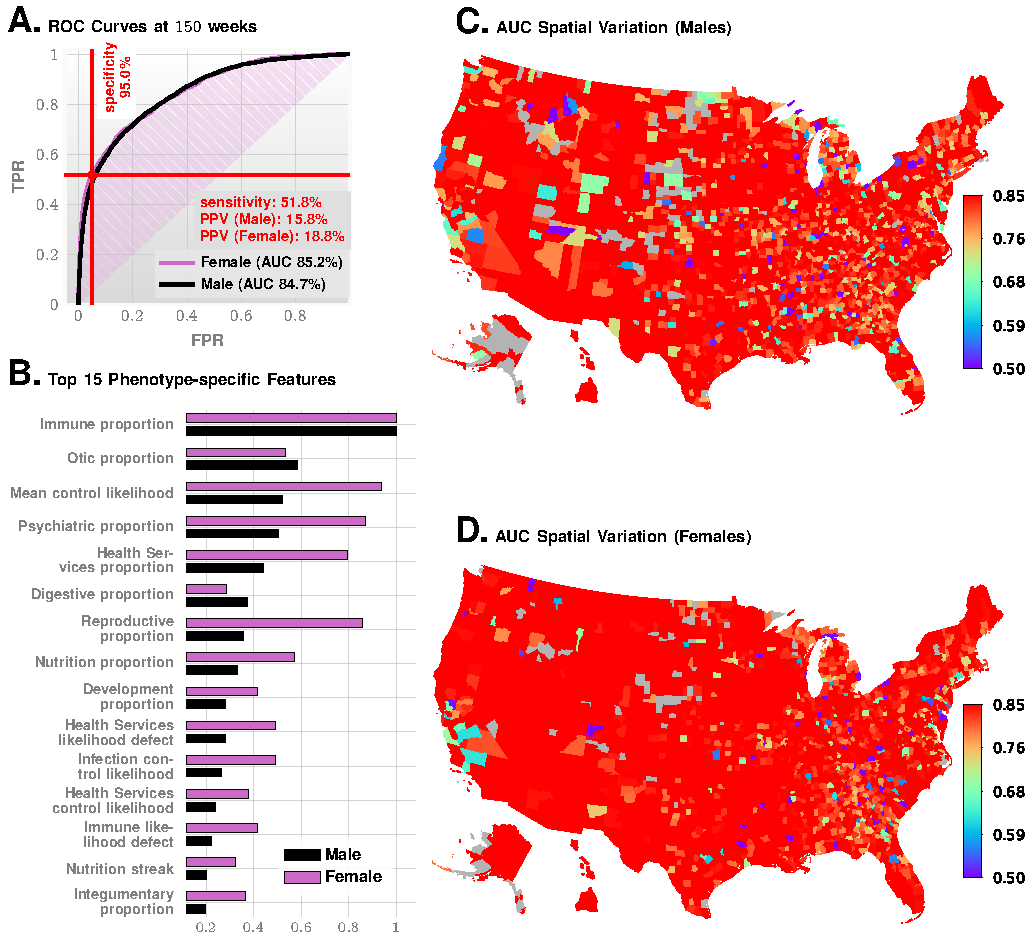
\includegraphics[width=0.8\textwidth]{Figures/main2-figure1.pdf}};

    \end{tikzpicture}
     \vspace{-10pt}

  \captionN{Panel A:  ROC curves. Panel B: feature importance inferred by our prediction pipeline. The most import feature is related to immunologic disorders, and we note that in addition to features related to individual disease categories, we also have the mean control likelihood (rank 3), which may be interpreted as the average likelihood of the diagnostic patterns in the control category vs the \treatment category. 
     }\label{fig1}
        \vspace{-15pt}

\end{wrapfigure}While the Truven database is used for both training and out-of-sample cross-validation with held-back patient data, our second independent dataset (referred to as the UCM dataset) consisting of de-identified diagnostic records for children treated at the University of Chicago Medical Center between the years of 2006 to 2018, aids in further cross-validation. We considered children between the ages of $0-5$ years, and  applied the same exclusion criteria as the Truven dataset.

Predicting  future ASD diagnosis   is a  binary classification problem: we classify time-stamped sequences of diagnostic codes  into \treatment and \control categories, where the ``\treatment'' category refers to patients eventually  diagnosed with ASD (defined as people with one or more ICD9/10 codes corresponding to ASD in their medical history). 
For learning the differences in longitudinal patterns, we consider  data from birth (or the earliest record) upto the time at which the prediction/screening is done.
We do not pre-select any diagnostic   code based on its  suspected comorbidity with ASD. 

\subsection*{Modeling \& Prediction}
The significant diversity of diagnostic codes, along with the sparsity of codes per patient (30-100 codes on average  per patient per year of life, with 9,835 unique codes leads to very few consistent repeats for straightforward  probability calculations)   makes this a difficult learning problem. 
We proceed by  partitioning the  disease spectrum into \DXphn\xspace broad  categories, $e.g.$ infectious diseases, immunologic disorders, and endocrinal disorders. Some of these categories comprises a relatively large number of diagnostic codes aligning roughly with the  ICD categories~\cite{hedegaard2019international}.   Each  category yield a single time series over weeks (each week being identified as having a value '0' for no code corresponding to the diagnostic category, or  '1' if some code is present, and '2' if a diagnostic code from any of the other categories is present). 
These time series are  compressed into specialized Hidden Markov Models known as Probabilistic Finite Automata~\cite{CL12g,Chattopadhyay20140826}. These models are inferred separately for each phenotype,  for each sex, and for the control and the \treatment cohorts,  to identify   distinctive average patterns  emerging at the population level. Thus, we infer 
$\DXphn\times 2 \times 2  = \the\numexpr  \DXphn  *2 *2  \relax$  PFSA models in total in this study. Variation in these inferred models across \treatment and \control groups  quantify the divergence of comorbidity patterns with increasing risk~\cite{huang2019data}. 

%#TODO NUMFEATURES
In addition, we use a range of engineered features that reflect various aspects of the patient-specific diagnostic histories, ultimately computing   $\numfeatures$  features    for each patient. These features are  used to train a standard gradient boosting classifier~\cite{ke2017lightgbm} aiming to  map   individual patients  to a raw risk score. $75\%$ of our patients are randomly selected for training with the rest  held-out as a validation set. We measure our performance using  standard metrics including the Area Under the receiver-operating characteristic curve (AUC), sensitivity, specificity, and  the Positive Predictive Value (PPV).

%\subsection*{Feature Importance \& Comorbidity Spectra}
Calculation of the \acor score offers  insights into the relative importance of  comorbidity categories, computed  by estimating the  mean change in the raw risk via random perturbation of a particular feature: this is the ``feature importance'' shown in Fig.~\ref{fig1}c for top contrubuting  categories, indicating that immunological, otic, digestive disorders and infections  are   important categories  modulating the \acor score. In our preliminary studies, we  found excellent disambiguation from other intellectual disabilities.


Importantly, our features are  based on data already  available in the past  medical records. We do not demand results from specific tests, or look for specific demographic, bio-molecular, physiological and other parameters; \textit{we use what we get} in the diagnostic history of patients.

% %####################################
\def\RCOL{\rowcolor{teal!40}}
% ####################################

% %####################################
The standalone performance in preliminary studies is summarized  in Figs.~\ref{fig1} and \ref{fig2}. 
We achieve an out-of-sample AUC of $82.3\%$ for males and $82.5\%$ for females at $125$ weeks of age for the Truven dataset. In the UCM dataset, our performance is comparable: $83.1\%$ and $81.3\%$ for males and females respectively at $125$ weeks of age. The good agreement of the out-of-sample performance on these independent datasets lends strong support for our claims. The specificity, sensitivity, PPV trade-offs are shown in Table~\ref{tabssp}. We enumerate the top $15$ predictive features in Fig.~\ref{fig1}B. 
We also computed the county-specific performance of the risk pipeline for the Truven dataset, and we got nearly uniform performance across the country for both genders. 
%
\begin{figure}[t]
 % \vspace{-15pt}
  
  \centering 
   \includegraphics[width=0.9\textwidth]{Figures/test-figure0}
   \vspace{-15pt}

    \captionN{Variation of Inferred Risk. Panel A illustrates AUC achieved as a function of
      patient age, for the Truven and UCM datasets: we achieve $>80\%$ AUC for either gender from shortly after 2 years.   Panel B illustrates  risk variation with time for the control and the positive cohorts. Panel C shows the distribution of the prediction horizon: the time to a clinical diagnosis after inferred  relative risk crosses $90\%$. Panel d illustrates the risk progression of a specific, ultimately autistic male child in the Truven database. }\label{fig2}
       \vspace{-15pt}

\end{figure}
%###########################################################
%
Fig.~\ref{fig2}A illustrates the variation of the  AUC  with increasing age of the subjects plotted with 99\% confidence bounds, indicating the predictive performance increases with age. We find that while the AUC gradients are slightly different in the two datasets are comparable.

%####################################
\begin{wraptable}[11]{l}{3in}  
  \centering
  \vspace{-19pt}
  
\captionN{Standalone \acor performance (M-CHAT/F: sensitivity=$38.8\%$,specificity=$95\%$, PPV=$14.6\%$)}\label{tabssp}
\fontsize{8}{8}\selectfont
  \vspace{-10pt}
 \begin{tabular}{L{.27in}|L{.27in}|L{.27in}|L{.25in}|L{.25in}|L{.45in}}
\hline
week&spec.&sens.&PPV&sex&dataset\\\hline
100&0.92&0.39&0.14&F&UCM\\\hline
100&0.95&0.39&0.19&M&UCM\\\hline
100&0.93&0.39&0.13&F&Truven\\\hline
100&0.91&0.39&0.10&M&Truven\\\hline
%\RCOL 112&0.94&0.35&0.17&F&UCM\\\hline
\RCOL 112&0.93&0.39&0.16&F&UCM\\\hline
\RCOL 112&0.95&0.39&0.20&M&UCM\\\hline
\RCOL 112&0.96&0.39&0.22&F&Truven\\\hline
\RCOL 112&0.95&0.39&0.17&M&Truven\\\hline
% 150&0.94&0.39&0.19&F&UCM\\\hline
% 150&0.98&0.39&0.34&F&Truven\\\hline
% 150&0.97&0.39&0.26&M&Truven\\\hline
% 150&0.97&0.39&0.26&M&UCM\\\hline

\end{tabular}
\end{wraptable}  
%####################################
We plot the raw risk over time for males and females for the out-of-sample control and \treatment cohorts in Fig.~\ref{fig2}B. Notably, averaged over the population,   the risks differ  from $50$ weeks showing that early diambiguation is possible. Guthrie $\etal$~\cite{pmid31562252}  has  demonstrated that  as a nearly universal screening tool (n=20,375) M-CHAT/F has a sensitivity of 38.8\%, specificity of 94.9\% and PPV of 14.6\%, which suggests  (See Table~\ref{tabssp}) that our approach produces a  superior PPV (exceeding M-CHAT/F PPV by at  $14\%$ (14.1-33.6\%) when sensitivity and specificity are held at comparable values around the age of 26 months ($\approx 112$ weeks). 

%#################################### 
\begin{wraptable}[9]{l}{4.2in}
  \centering
  \vspace{-18pt}
  
\captionN{Boosted Sensitivity, specificity and PPV at  26 months with \acor  Conditioned on M-CHAT/F Scores}\label{tabboost}
\fontsize{8}{8}\selectfont

\vspace{-10pt}

\begin{tabular} {L{.2in}|L{.2in}|L{.2in}|L{.2in}||L{.275in}|L{.285in}|L{.285in}||L{.275in}|L{.285in}|L{.285in}}
\hline
\multicolumn{4}{c||}{\cellcolor{lightgray!60}M-CHAT/F Outcome}  & \multicolumn{3}{c||}{\mnp{.9in}{\vskip .2em  perf. (Truven)\vskip .2em  } }&\multicolumn{3}{c}{\mnp{1in}{\vskip .2em  perf. (UCM)\vskip .2em }} \\\cline{0-9}
 0-2  NEG & 3-7  NEG & 3-7  POS & $\geq  8$  POS & \multirow{2}{*}{\mnp{.1in}{speci-ficity}} & \multirow{2}{*}{\mnp{.1in}{sensi-tivity}} &\multirow{2}{*}{PPV}& \multirow{2}{*}{\mnp{.1in}{speci-ficity}} & \multirow{2}{*}{\mnp{.1in}{sensi-tivity}} & \multirow{2}{*}{PPV}  \\\cline{0-2}
\multicolumn{4}{c}{\cellcolor{lightgray} specificity choices}  & & & &&&\\\hline 
  0.2&0.54&0.83&0.98&0.95&0.585&0.209&0.95&0.505&0.186&0.022\\\hline 
0.21&0.53&0.83&0.98&0.95&0.586&0.208&0.95&0.506&0.184&0.022\\\hline 
0.42&0.87&0.98&0.99&\cellcolor{\PCOL}0.98&\cellcolor{\PCOL}0.433\cellcolor{\PCOL}&\cellcolor{\PCOL}0.331&0.98&0.347&0.284&0.022\\\hline 
0.48&0.87&0.97&0.99&\cellcolor{\PCOL}0.98&\cellcolor{\PCOL}0.432&\cellcolor{\PCOL}0.331&0.98&0.355&0.289&0.022\\\hline 
0.38&0.54&0.94&0.98&\cellcolor{\PCOL}0.95&\cellcolor{\PCOL}0.736\cellcolor{\PCOL}&\cellcolor{\PCOL}0.203&0.95&0.628&0.178&0.017\\\hline 
0.3&0.55&0.94&0.98&\cellcolor{\PCOL}0.95&\cellcolor{\PCOL}0.737&\cellcolor{\PCOL}0.203&0.95&0.633&0.179&0.017\\\hline 
0.58&0.96&0.98&0.99&0.98&0.492&0.302&0.98&0.373&0.247&0.017\\\hline 
0.59&0.96&0.98&0.99&0.98&0.491&0.303&0.98&0.372&0.248&0.017\\\hline 
0.46&0.92&0.97&0.99&0.977&0.534&0.291&0.977&0.448&0.256&0.017\\\hline 
0.48&0.92&0.97&0.99&0.978&0.533&0.292&0.978&0.448&0.257&0.017\\\hline 
 
\end{tabular}
\vspace{-18pt}

\end{wraptable}  
%####################################
Ultimately, depending on Aim 2, we would attempt to combine \acor amd M-CHAT/F  via a conditional choice of  sensitivity/specificity trade-offs. In our preliminary studies, this boosts overall performance significantly, with  a PPV $\approx 30\%$  across datasets, or a sensitivity close to or exceeding $50\%$, when we restrict specificities to above $95\%$ (See Table~\ref{tabboost}). 

\subsection*{Research Design}
\ZERO methodology can  screen instantaneously   every child  in primary care, for whom past medical history is available, with zero administrative and resource burden. To achieve the specific  aims, we will gather data from both the child and the primary caregiver in the participating  primary care clinic. The key steps are as  follows (See Fig.~\ref{figflow}):
%#TODO AGE RESTRICTION
\begin{enumerate} 
[label=$\square$, leftmargin=0pt,
labelindent=0em, topsep=0.1em, labelsep=*, itemsep=.5em,itemindent=1em]
 \item 1. Pediatric clinic team  will  adminster  M-CHAT/F to incoming children with 16-30 months.
\item 2. The PI's team will
  compute  individual \acor  with consent (steps 1 and 2 in Fig.~\ref{figflow}).
\item 3. On being flagged by M-CHAT/F  as high risk, or if the \ZERO score indicates high risk and  M-CHAT/F is borderline,  the patients will be scheduled for ADOS-2 evaluation overseen by Dr. Smith and his team (Step 3 in in Fig.~\ref{figflow}).
\item 4. The evaluation scores will be analyzed by  PI and his  team.
\end{enumerate}

\begin{wrapfigure}[24]{l}{2.5in}
  \vspace{-30pt}
  
  \hspace{-10pt}\includegraphics[width=2.75in]{Figures/flow1}
  \vspace{-25pt}
  
  \caption{Patient processing logic }\label{figflow}
\end{wrapfigure}
The limited scope of this project implies that we need to be aware of the number of ADOS-2 refrerreal generated due to \ZERO, particularly since ADOS-2 evaluations involve significant resource and cost.

\subsection*{Cohort Selection}

Participants (16-26 months) will be approximately 5000 children per year (producing approximately 300 ADOS-2 referrals from M-CHAT/F at no cost to the project) who will be evaluated via both the MCHAT-F screening  during wellness visits at the 1 year, 1.5 year and 2 year mark, and the \ZERO algorithm applied to their diagnostic history on file. Additional inclusion criteria: Child has diagnostic history on record with at least 5 diagnostic codes, and the first code is at least from 15 weeks in the past. Additional exclusion criteria: Diagnostic history only consists of health service contact codes.

Beyond the evaluation of $\approx 300$ children as a part of standard clinical workflow, we will evaluate $100-120$ children at no cost to the patient family, to evaluate the efficacy of \acor when M-CHAT/F is borderline (and does not trigger downstream diagnostic evaluation by itself).

\subsection{Study Interventions}
No intervention is planned. Outcomes are  efficacy and applicability of \ZERO.
\subsection*{Risk To Patients} The design of the study guarantees that patients suffer no negative impact from the added \ZERO screen. Indeed, persuant to available resources, patients might  be expedited for ADOS evaluation which  reduces their wait-times. For some borderline cases, which would have been missed by M-CHAT/F, might get flagged by \ZERO, and be scheduled for ADOS, which they would not have had to do with just M-CHAT/F. But this is a positive outcome. There is a small possibility  that \ZERO, due to its own false positives  different from that of M-CHAT/F, might schedule some children for ADOS, who do not have autism, and might cause some stress in parents and families if they are . The potential societal benefit gained in lieu of this discomfort is the validation of the expected  performance boost for ASD screening at the population level PPV by up to 100\%, or the sensitivity by 50\%.

\subsection*{Procedures} Eligible patients at the Department of Pediatrics, University of Chicago (patients who present for a well-child visit or any other non-emergency reason) will be asked  for consent for access to their past medical history for carrying out the \ZERO screen. 
If there is a flag either in M-CHAT/F or if M-CHAT/F is borderline with a flag in \ZERO, the  pediatrician will inform parents of a potential elevated risk of ASD, and offer to schedule for an ADOS-2 evaluation. 
The ADOS-2 evaluation triggered by \ZERO flags will be at no cost to the patient.

 All study procedures and consent forms will be approved by the University of Chicago Institutional Review Board.  For all assessments, basic demographic information, recruitment site, medications and diagnoses assigned by the current clinical treatment team, will be obtained from the parent/caregiver and medical record.

\subsection*{Data Management} Data collection forms for demographic and clinical history data, database design and data management procedures will be designed, created and conducted at the University of Chicago under the
direction of Dr. Smith and Prof. Chattopadhyay. Demographic and clinical history data will be collected and entered into an HIPAA compliant secure database.  Monthly reports will be generated  to monitor data timeliness, completeness, and accuracy as well as subject flow through the study. 


\clearpage

\bibliographystyle{naturemag}
\bibliography{aut,BibLib1}

\end{document}


% LocalWords:  neurobiological morbidities modality
 